\documentclass[12pt, twoside, hidelinks]{report}
\usepackage[T1]{fontenc}
\usepackage[polish] {babel}
\usepackage{hyperref}
\usepackage[left = 1in, right = 1in, top = 1in, bottom = 1in]{geometry}
\usepackage{eso-pic}
\newcommand\BackgroundPic{%
\put(0,0){%
\parbox[b][\paperheight]{\paperwidth}{%

\includegraphics[width=\paperwidth,height=\paperheight]{A4h.jpg}
}}}
\usepackage{xcolor}
\usepackage{secdot}
\usepackage{graphicx}
\usepackage{wrapfig}
\usepackage{fancyhdr}
\pagestyle{fancy}
\fancyhf{}
\fancyhead[LE,RO]{\rightmark}
\fancyfoot[LE,RO]{\thepage}
\fancyfoot[RE,LO]{\leftmark}
\renewcommand{\headrulewidth}{0.5pt}
\renewcommand{\footrulewidth}{0.5pt}
\usepackage[left = 1in, right = 1in, top = 1in, bottom = 1in]{geometry}
\usepackage{helvet}
\renewcommand{\familydefault}{\sfdefault}
\renewcommand{\labelitemi}{\textendash}
\renewcommand{\labelenumi}{\Roman{enumi}}
\raggedbottom
\title{}
\author{Grzegorz Smoliński}
\date{}
\begin{document}
\AddToShipoutPicture*{\BackgroundPic}
\begin{titlepage}
\null\vfill\vskip 2cm

  \begin{flushleft}
  
  {\Huge \textcolor{white}{Instrukcja do ,,Bazy rolników''}\par}
  \vskip 1.5cm

  {\Large \textcolor{white}{Grzegorz Smoliński}\par}
  \vskip 1cm

  {\large}
  \end{flushleft}

\vfill
\vfill
\end{titlepage}
\tableofcontents
\thispagestyle{empty}
\listoffigures
\thispagestyle{empty}
\pagebreak
\pagenumbering{arabic}
\chapter{Odczyt}
\thispagestyle{empty}
\pagebreak
\section{Wyszukiwanie zmiennych i pobieranie ich opisu}
Aplikacja ,,Baza rolników'' ma w zamierzeniu dawać użytkownikowi dużą swobodę w tym, jakimi zmiennymi chce opisywać kontakty w bazie. Z tego powodu zmienne, z niewielkimi wyjątkami, nie są predefiniowane. Sprawia to równocześnie, że po stronie użytkownika leży odpowiedzialność, by zmienne miały jasne znaczenie i nie powtarzały informacji (nie obciążały niepotrzebnie bazy danych). \par
\begin{figure}[h!]
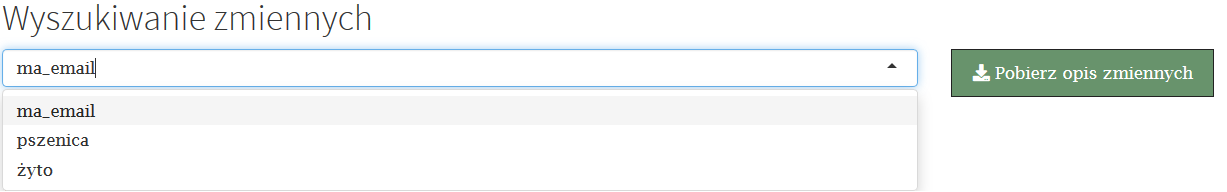
\includegraphics[width = 1\textwidth]{1.1.}
\caption{Interfejs do wyszukiwania zmiennych i pobierania ich opisu.}
\label{wyszukiwanie_zmiennych_i_pobieranie_ich_opisu_interfejs}
\end{figure}
Rozwijana lista (rys. \ref{wyszukiwanie_zmiennych_i_pobieranie_ich_opisu_interfejs}) pozwala podejrzeć wszystkie zmienne stworzone przez użytkownika. Program przy każdym imporcie danych tworzy zmienną ,,ma\textunderscore email'', która również znajduje się na tej liście. Zmienna ta mówi o tym, czy kontakt posiada adres e-mail (,,Tak''/,,Nie''), sprawdzając, czy w miejscu adresu e-mail podano nazwę składającą się ze znaku ,,@''. \par
Aplikacja wykorzystuje ponadto dwie dodatkowe zmienne: status i województwo, które nie znajdują się na liście, ponieważ filtrowanie za ich pomocą odbywa się w inny sposób - nie poprzez ręczne wpisywanie ich do pól z warunkiem filtrującym, ale wybór statusów i województw z listy poniżej pól do wpisywania warunku filtrującego. \par
Po prawej od rozwijanej listy ze zmiennymi znajduje się przycisk, za pomocą którego można pobrać bardziej szczegółowe informacje o wszystkich zmiennych z listy. Oprócz nazwy, jest to etykieta (opis zmiennej, który stworzył użytkownik) oraz wartości, jakie zmienna obecnie przyjmuje (czyli te, które rzeczywiście występują w bazie danych). Dla zmiennych jakościowych wszystkie wartości zostaną wypisane, natomiast dla zmiennych ilościowych będzie to wartość minimalna i maksymalna. Pobrany zostanie plik Excel (rys. \ref{pobrany_opis_zmiennych}).
\begin{figure}[h!]
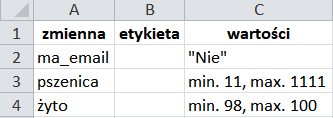
\includegraphics[width = 0.5\textwidth]{1.5.}
\centering
\caption{Pobrany opis zmiennych.}
\label{pobrany_opis_zmiennych}
\end{figure}
\section{Filtrowanie i odczyt bazy}
\begin{figure}[h!]
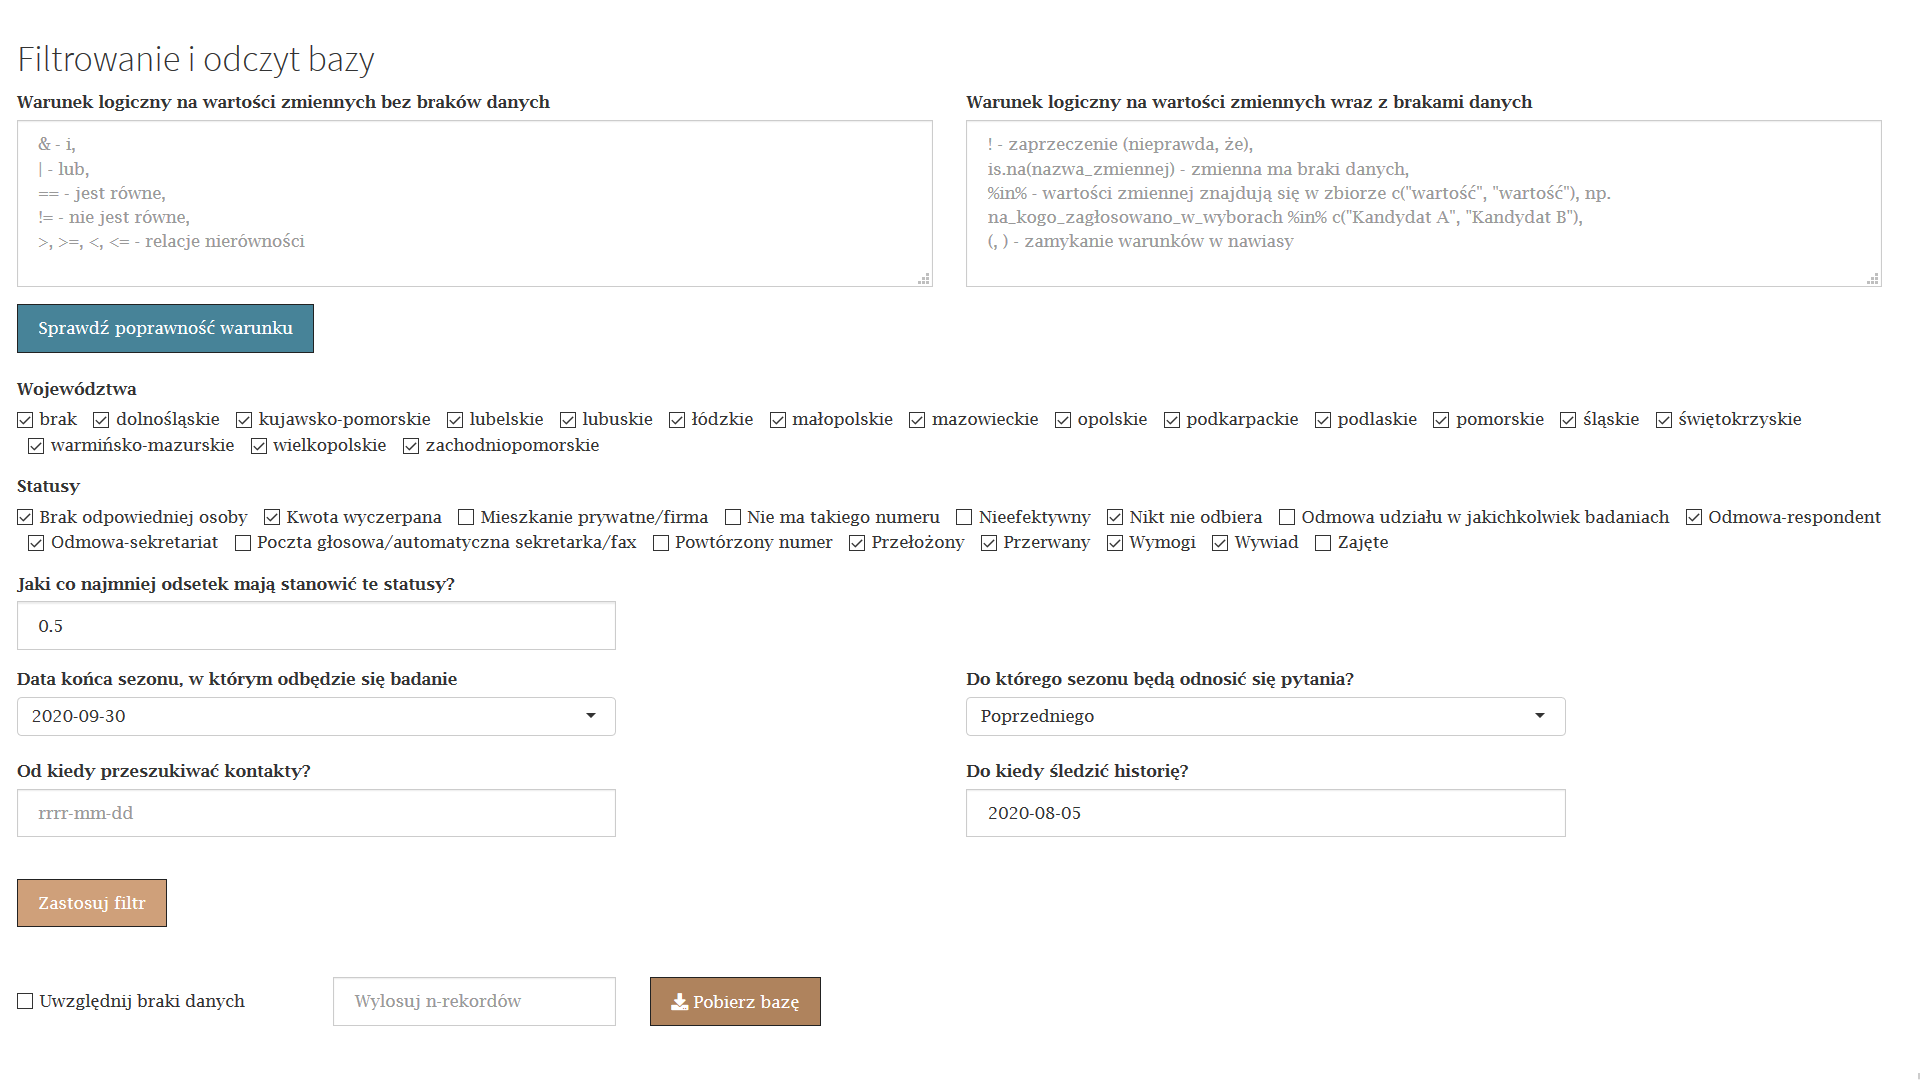
\includegraphics[width = 1\textwidth]{1.2.}
\caption{Interfejs do filtrowania i odczytu bazy.}
\label{filtrowanie_i_odczyt_bazy_interfejs}
\end{figure}
Filtrowanie bazy danych opiera się na (1) rozróżnieniu pomiędzy zmiennymi widocznymi na liście zmiennych a statusem i województwem; (2) rozróżnieniu pomiędzy wynikami filtrowania niezawierającymi braków danych i zawierającymi je; (3) określeniu czasu dla wyszukiwanych informacji, w tym określeniu, czy program powinien zwracać dane historyczne, tzn. dane, o których wiadomo, że dla danego kontaktu są inne niż dane późniejsze. Interfejs do filtrowania i odczytu bazy przedstawia rys. \ref{filtrowanie_i_odczyt_bazy_interfejs}. \par
Filtrowanie oraz odczyt bazy składa się z osobnych etapów wyznaczanych przez przyciski ,,Zastosuj filtr'' oraz ,,Pobierz bazę'', w takiej właśnie kolejności. Zatem, aby móc pobrać bazę, trzeba wcześniej określić, jaki jej fragment jest potrzebny. Nie jest możliwe pobranie całej bazy, choć możliwe jest wyświetlenie wielkości całej bazy z podziałem na województwa - stanie się tak, jeśli w polu ,,Warunek logiczny na wartości zmiennych bez braków danych'' nic nie zostanie wpisane lub wpisany filtr będzie miał błędy, a mimo to użyje się przycisku ,,Zastosuj filtr''. \par
Pierwszym etapem stworzenia filtru jest wypełnienie co najmniej pola ,,Warunek logiczny na wartości zmiennych bez braków danych'' tekstem o poprawnej składni. Poprawność jest wyznaczana poprzez spełnienie następujących warunków:
\begin{itemize}
\item zastosowano wyłącznie zmienne, które znajdują się na liście ,,Wyszukiwanie zmiennych''
\item zmienne te, jeśli występuje ich więcej niż jedna, łączone są za pomocą dozwolonych spójników logicznych, tj. ,,i'' bądź ,,lub''
\item w polu ,,warunek logiczny na wartości zmiennych bez braków danych'' nie posłużono się składnią, która pozwala wyszukiwać braki danych, czyli ,,is.na(nazwa\textunderscore zmiennej)''
\item zawężanie wartości zmiennej odbywa się za pomocą poprawnych funkcji, jak np. jest równe (==), nie jest równe (!=)
\end{itemize}
W obu polach ,,Warunek logiczny...'' wypisane są elementy, których można użyć, budując wyrażenie filtrujące. Za wyjątkiem ,,is.na(nazwa\textunderscore zmiennej)'', wszystkie je można wykorzystywać w dowolnym polu. Poniżej przedstawiono przykłady poprawnych wyrażeń:
\begin{center}
pszenica > 5 \& żyto>50
\end{center}
Szukamy tych, którzy mają więcej niż 5 ha pszenicy i więcej niż 50 ha żyta. Nie ma znaczenia, w jakich miejscach zastosujemy bądź nie spacje.
\begin{center}
(pszenica > 5 \& żyto > 50) | ma\textunderscore email == "Tak"
\end{center}
Do poprzedniego warunku dodajemy - ,,lub zmienna ma\textunderscore email przyjmuje wartość ,,Tak''''. Należy zauważyć, że (1) nawiasy mają znaczenie - jeśli ktoś nie ma więcej niż 5 ha pszenicy i 50 ha żyta, ale posiada email, to zostanie wyszukany; (2) w przypadku zmiennej jakościowej, wartości, które nas interesują, muszą być wypisane z użyciem cudzysłowu angielskiego (górnego).\par
W powyższym przypadku nie było konieczne zastosowanie nawiasów - najpierw jest bowiem zawsze ewaluowany spójnik ,,i'', a dopiero później ,,lub''. Wcześniej od ,,i'' jest ewaluowane zaprzeczenie (,,!'').
\begin{center}
(pszenica > 5 \& żyto > 50) | (is.na(pszenica) \& is.na(żyto))
\end{center}
Szukamy tych, którzy mają więcej niż 5 ha pszenicy i więcej niż 50 ha żyta lub są w bazie, lecz nie ma informacji o tym, ile mają pszenicy i ile mają żyta.
\begin{center}
(pszenica > 5 \& żyto > 50) | is.na(pszenica) | is.na(żyto)
\end{center}
Szukamy tych, którzy mają więcej niż 5 ha pszenicy i więcej niż 50 ha żyta lub są w bazie, lecz nie ma informacji o tym, ile mają pszenicy lub ile mają żyta. \par
Jeśli chcemy w wynikach wyszukiwania otrzymać również te osoby, dla których istnieją braki danych, powinniśmy trzymać się pewnych dodatkowych warunków:
\begin{itemize}
\item w polu ,,Warunek logiczny na wartości zmiennych wraz z brakami danych'' nie może pojawić się zmienna, która nie pojawiła się w polu ,,Warunek logiczny na wartości zmiennych bez braków danych''
\item nie jest możliwe, aby ta sama osoba miała np. informację o areale pszenicy i jednocześnie nie miała takiej informacji, czyli w przypadku braków danych należy używać spójnika ,,lub'' wtedy, gdy dotyczy to tej samej zmiennej
\end{itemize}
Program daje częściowo możliwość sprawdzenia, czy utworzony przez nas warunek jest poprawny. Oczywiście, nie da się sprawdzić, czy jest on zgodny z intencją użytkownika, ale pozwala wykryć błędy składniowe, takie jak: niepoprawna nazwa zmiennej czy użycie funkcji, która nie istnieje lub nie może być wykorzystana do filtrowania. Służy do tego przycisk ,,Sprawdź poprawność warunku''. Zwraca on trzy rodzaje wyników - puste, jeśli nie ma czego sprawdzać; ,,OK'', jeśli wszystko jest poprawne; lub ogólną informację, że występuje błąd. \par
W dalszej kolejności trzeba wybrać województwa, które chcemy przeszukiwać oraz określić, jakie statusy będą brane pod uwagę. Statusy to rezultaty wcześniej wykonywanych połączeń. \par
O ile kwestia województw nie wymaga dalszych wyjaśnień, o tyle przeszukiwanie statusów wiąże się z różnymi rozwiązaniami, o których użytkownik powinien wiedzieć. Po pierwsze, dla każdego kontaktu przechowywanych jest maksymalnie dwadzieścia ostatnich statusów. Po drugie, wyszukiwanie opiera się na tym, że określa się, jaki odsetek interesujące nas statusy mają stanowić spośród wszystkich, które przynależą do danego kontaktu. Oba te kryteria można modyfikować: wybierać statusy wedle uznania oraz ustalać minimalny dla nich odsetek w odpowiednim polu. Domyślnie wybrano statusy wskazujące na to, że ktokolwiek odezwał się podczas próby kontaktu (oraz nie zakończyło się to informacją o tym, że numer prowadzi pod zły adres) i ustawiono minimalny odsetek tych statusów na 0,5. Jeśli jako minimalny odsetek wpisałoby się coś, co nie jest liczbą lub wartość większą niż 1 bądź mniejszą niż 0, to program przeformułuje ją na 0,5.\par
Ostatnim elementem stanowiącym kryterium wyszukiwania jest czas. Określa się go za pomocą czterech pól: dwa pierwsze odnoszą się do tego, kiedy będzie miało miejsce badanie oraz jaki okres będzie nas w tym badaniu interesował (tj. do którego sezonu będą odnosić się pytania kwalifikujące do badania), dwa kolejne pola dotyczą tego, od kiedy wyszukiwać rekordy w bazie oraz, jak daleko sięgać do historii każdego z kontaktów. \par
Program wszystkie daty w przypadku filtrowania zaokrągla do sezonów. Sezon to okres od początku października do końca września. Oparcie się na sezonach oznacza, że dla danego kontaktu przechowywana jest, dla danej zmiennej, tylko jedna wartość z danego sezonu, aktualizowana na podstawie daty badania, tzn. wartość najnowsza. Jeśli przeprowadzono badanie 2020-04-04, w którym respondenta X zapytano o areał pszenicy i o to samo pytano tego samego respondenta 2020-05-05, to zachowana zostanie jedynie wartość z badania 2020-05-05, ponieważ obie te daty przynależą do tego samego sezonu.  \par
Naturalniejsze wydaje się jednak myślenie o datach bez konieczności zaokrąglania ich w głowie do sezonów, dlatego zakłada się, że użytkownik będzie wprowadzał rzeczywiste daty, które go interesują, a program sam zaokrągli je do sezonów. Zaokrąglanie do sezonów odbywa się poprzez wyznaczenie ostatniego dnia sezonu, do którego należy data, czyli za każdym razem będzie to trzydziesty września, zmieniać będzie się jedynie rok. \par
Pierwszą rzeczą, którą należy ustalić w trakcie filtrowania, jeśli chodzi o daty, jest to, jaki sezon będzie nas interesował. Możliwe są dwa warianty - w przypadku pola dotyczącego sezonu, w którym odbędzie się badanie, może to być obecny sezon lub przyszły (wyznaczany przez datę z ostatnim dniem danego sezonu). W przypadku sezonu, do którego będą odnosić się pytania, do wyboru jest sezon obecny lub poprzedni (wyznaczany przez opcje ,,Obecnego'' lub ,,Poprzedniego''). Chodzi tu, oczywiście, o to, jaka będzie konstrukcja pytania w kwestionariuszu w stosunku do tego, w którym sezonie odbywa się badanie. \par
Następnym kryterium jest to, od kiedy dane uznajemy za interesujące, a kiedy są już tak stare, że nie mają dla nas znaczenia. Wyznacza to pole ,,Od kiedy przeszukiwać kontakty?''. Domyślnie nie ma ustawionej wartości, ale jeśli pozostanie puste lub jeśli wpisze się datę o niepoprawnym formacie, przeszukiwanie będzie się odbywać od roku 1970-01-01 zaokrąglonego do sezonów. Pole to, wyznaczając, od kiedy dane mają dla nas wartość, wyznacza tym samym, od kiedy dane przestajemy traktować jako brak danych. Jeśli przeszukujemy bazę od roku 2015, a istnieje kontakt, który posiada informacje o areale pszenicy wyłącznie dla roku 2014, to kontakt ten będzie traktowany jako taki, który wcale nie posiada informacji o areale pszenicy, a więc da się go wyszukać wyłącznie wtedy, gdy interesować nas będą również braki danych dla pszenicy. \par
Kolejna data to wartość wpisana w pole ,,Do kiedy śledzić historię?''. Przyjęto tu założenie, że użytkownik może chcieć wyszukać kontakt, w przypadku którego dane historyczne spełniają warunek filtru, ale dane nowsze nie spełniają, np. chcemy otrzymać osoby uprawiające ponad 5 ha pszenicy; dana osoba uprawiała ponad 5 ha pszenicy w sezonie 2016/2017, ale mniej niż 5 ha pszenicy w sezonie 2017/2018 i brak późniejszych danych o pszenicy dla tego kontaktu. W kilku przypadkach wyszukiwanie, mimo odpowiednich ustawień, może nie odnaleźć takiego kontaktu, np. jeśli w obecnym sezonie wiadomo, że osoba ta ma 5 ha pszenicy lub mniej i badanie, dla którego szukamy respondentów, odbędzie się w obecnym sezonie itp. w zależności od tego, jak ustawione zostały pola dot. tego, w którym sezonie badanie się odbędzie i do którego sezonu będą odnosić się pytania.  \par
Myśląc o ustalaniu dat dla filtrowania, należy myśleć o tym jak o odrzucaniu informacji. Wyznaczamy datę początkową - od tej daty wartości zmiennych są dla nas interesujące oraz wyznaczamy datę końcową - jest to data tego, do którego sezonu będą odnosić się pytania w badaniu, do którego szukamy respondentów. Ten horyzont czasowy służy jednocześnie do określania ciągłości czasowej dla danych - respondent, dla którego mamy informacje o areale pszenicy w 2018 r., ale nie dla roku 2019 ani 2020, a jednocześnie szukamy od roku 2017 i interesuje nas sezon kończący się dnia 2020-09-30 (w tym sezonie odbędzie się nasze przyszłe badanie), nie będzie traktowany jako ktoś, kto ma brak danych dla sezonu 2020. Program przyjmie, że respondent ten uprawia tyle samo pszenicy, co w ostatnim sezonie, dla którego - w ramach przyjętego horyzontu czasowego - ma informacje. W tym wypadku będzie to rok 2018. Kierunek przyjmowania wartości biegnie najpierw od przeszłości do przyszłości, a później odwrotnie, tj. gdyby w naszym przypadku respondent miał informacje o areale pszenicy w 2020, a my szukalibyśmy danych dla 2019, to program przyjąłby, że respondent w 2019 miał tyle samo pszenicy, co w 2018. Gdyby od roku 2017 nie było informacji o areale pszenicy dla tego respondenta, to program przyjąłby, że w roku 2019 respondent ten miał tyle samo pszenicy, co w roku 2020. \par
Oznacza to tym samym, że wspomniany respondent nie jest przykładem osoby, dla której nie mamy danych dla roku 2019. Byłby takim przykładem tylko wtedy, jeśli w wyznaczonym horyzoncie czasowym nie mielibyśmy żadnych informacji o areale pszenicy dla tego respondenta. \par
Wypełnianie brakujących wartości dla zmiennych tam, gdzie to możliwe, sprawia jednocześnie, że czasem w wynikowej bazie danych mogą pojawić się wartości zmiennej pochodzące z horyzontu czasowego, który nas nie interesował. Przyjęto bowiem np., że nawet jeśli nie interesuje nas sezon kończący się 2020-09-30, tylko 2019-09-30, ale dla danego kontaktu istnieją dane za 2020-09-30, to one mogą być użyte do wypełniania braków danych wtedy, gdy nie ma danych z przeszłości (,,odciętej'' przeszłości). To nie działa jednak w przypadku odcinania od dołu, tj. szukaniu od określonej daty. \par
Poniżej zamieszczono wynik zapytania ,,pszenica > 5'' dla pola bez braków danych oraz zapytania ,,pszenica > 5 | is.na(pszenica)'' dla pola z brakami danych (rys. \ref{wynik_filtrowania}). \par
\begin{figure}[h!]
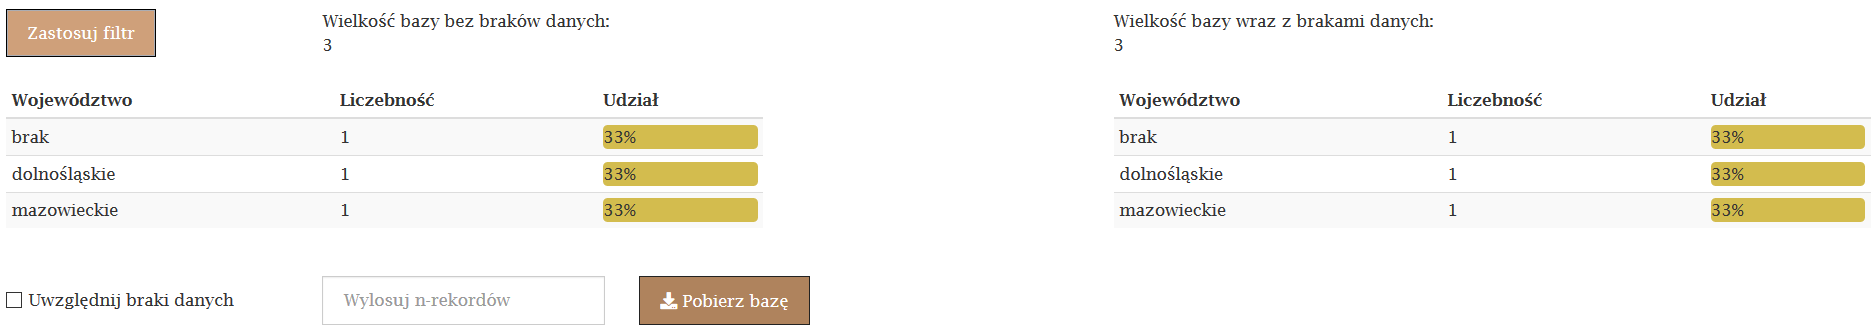
\includegraphics[width = 1\textwidth]{1.3.}
\caption{Wynik filtrowania.}
\label{wynik_filtrowania}
\end{figure}
Wyświetlenie osobnych zestawień dla wyników bez i z brakami danych pozwala porównywać, dla którego zapytania otrzymano satysfakcjonującą liczebność. Tabele są posortowane rosnąco względem liczebności. Aby pobrać bazę, wystarczy nacisnąć przycisk ,,Pobierz bazę'', choć wcześniej można jeszcze określić, czy uwzględnić braki danych (domyślnie: nie) oraz - jeśli nie chcemy pobierać wszystkich rekordów - ile z nich wylosować (losowanie spośród wyników z brakami danych lub bez, w zależności od tego, co zostało wybrane). Plikiem wynikowym jest plik Excel o postaci widocznej na rys. \ref{wyglad_pobranej_bazy}. \par
\begin{figure}[h!]
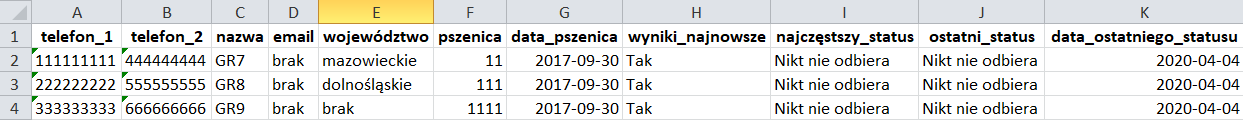
\includegraphics[width = 1\textwidth]{1.4.}
\caption{Pobrana baza.}
\label{wyglad_pobranej_bazy}
\end{figure}
Nie wszystkie elementy są tu stałe - liczba kolumn z telefonami może się zmieniać w zależności od tego, jak rzeczywiście wygląda baza danych oraz może być więcej kolumn ze zmiennymi stworzonymi przez użytkownika (zależą one od tego, co rzeczywiście było wyszukiwane). Stałe elementy to natomiast: telefon\textunderscore 1, nazwa, email, województwo, zmienna i data\textunderscore zmienna, wyniki\textunderscore najnowsze,  najczęstszy\textunderscore status, ostatni\textunderscore status, data\textunderscore ostatniego\textunderscore statusu. Data zmiennej to zawsze ostatni dzień sezonu, dla którego te dane zostały zebrane. Kolumna wyniki\textunderscore najnowsze określa, czy w przypadku tego kontaktu mamy do czynienia z danymi historycznymi, tj. czy istniały nowsze dane, które nie spełniały warunku filtrowania - jeśli nie, wtedy są to wyniki najnowsze. Informacje na temat statusów mogą być pomocne w celu określenia, które kontakty powinny lepiej rokować. Najczęstszy status jest wybierany losowo wtedy, gdy więcej niż jeden był najczęstszy. Daty statusów nie są zaokrąglane do sezonów, dlatego w tym przypadku otrzymujemy precyzyjniejszą informację, kiedy dana osoba ostatni raz wzięła udział w badaniu (jest to data przypisana do określonego badania, a nie dokładna data, kiedy rozmawiano z respondentem).
\chapter{Modyfikacja kontaktów}
\thispagestyle{empty}
\pagebreak
\section{Importowanie danych do bazy}
Aplikacja ,,Baza rolników'' służy do gromadzenia i wyszukiwania kontaktów, które - zanim znalazły się w bazie - zostały wykorzystane w badaniu. Taka konstrukcja programu sprawia, że nie jest wspierane importowanie do bazy kontaktów nigdy niewykorzystanych, do których nie próbowano jeszcze dzwonić. \par
\begin{figure}[h!]
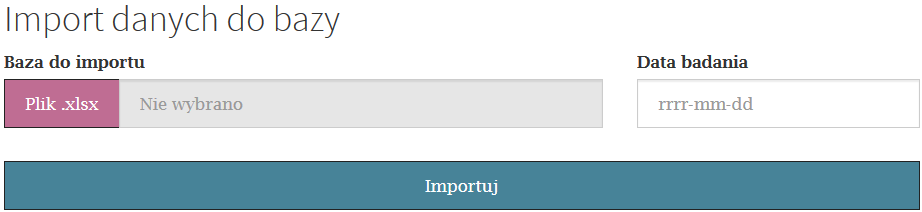
\includegraphics[width = 1\textwidth]{2.1.}
\caption{Interfejs do importowania danych do bazy.}
\label{importowanie_danych_do_bazy_interfejs}
\end{figure}
Poniżej znajdują się warunki, jakie spełnić musi importowany plik, by został zaakceptowany:
\begin{itemize}
\item plik Excel o rozszerzeniu .xls lub .xlsx
\item data badania w odpowiednim formacie, taka, która nie występuje jeszcze w bazie (tj. nie zaimportowano wcześniej badania o takiej dacie przeprowadzenia)
\item wymagane są kolumny: ,,telefon\textunderscore 1'', ,,nazwa'', ,,email'', ,,województwo'', ,,status''
\item nazwy kolumn, rozumiane jako nazwy zmiennych stworzone przez użytkownika, mogą zawierać tylko litery, cyfry i podkreślenia
\item nie można nazwać żadnej kolumny ,,telefon\textunderscore 0'' oraz liczby w nazwach kolumn z telefonami nie mogą być dwucyfrowe
\item każdy kontakt musi mieć przypisany status z puli dozwolonych statusów
\item każdy kontakt musi mieć przypisane województwo tylko z puli wszystkich województw w Polsce lub ewentualnie mieć słowo ,,brak''
\item w kolumnie ,,telefon\textunderscore 1'' możliwe są wyłącznie numery dziewięciocyfrowe lub numery dziewięciocyfrowe, po których następuje spacja, a dalej może być dowolna treść
\item w kolejnych kolumnach z telefonami możliwe są wyłącznie numery dziewięciocyfrowe lub numery dziewięciocyfrowe, po których następuje spacja, a dalej może być dowolna treść lub też dozwolone jest samo słowo ,,brak''
\item w kolumnach ,,nazwa'' oraz ,,email'' nie są dozwolone puste komórki. Jeśli zachodzi konieczność wskazania braków danych, to należy wpisywać odpowiednie określenie, np. ,,brak''
\item w kolumnie ,,telefon\textunderscore 1'' nie może być dubli
\item w importowanej bazie nie może być mniej kolumn z telefonami niż występuje w bazie rolników
\item liczby w nazwach kolumn z telefonami muszą być w kolejności rosnącej oraz przyrastać o 1
\item numery telefonów dla danego kontaktu nie mogą się powtarzać, tj. dany numer nie może występować w więcej niż jednej kolumnie z telefonem dla tego samego kontaktu
\item jeśli w danej kolumnie z telefonem występuje samo słowo ,,brak'', to na wszystkich kolejnych kolumnach z telefonem dla tego kontaktu musi również występować słowo ,,brak''
\item w zmiennych stworzonych przez użytkownika, tj. w kolumnach innych niż tych z numerami telefonów, nazwą, emailem, statusem i województwem nie może występować samo słowo ,,brak'', ponieważ ono nie będzie poprawnie interpretowane przez program jako brak danych. W takich kolumnach należy pozostawić pustą komórkę w przypadku braków danych
\end{itemize}
W jednym z warunków była mowa o tym, że w nazwach kolumn, które miałyby być nazwami zmiennych tworzonymi przez użytkownika, można używać wyłącznie liter, liczb i podkreślenia. Jest to prawda, o ile rozumieć to jako ograniczenie na nazwę zmiennej (tj. nazwę, która później będzie się wyświetlać na liście zmiennych). Sytuacja jest jednak bardziej skomplikowana, jeśli rozumieć to jako tekst, który zostanie wpisany do kolumn w importowanej bazie, które odzwierciedlają zmienne stworzone przez użytkownika. Dochodzi tu bowiem jeszcze jeden warunek:
\begin{itemize}
\item w importowanej bazie, w nazwach kolumn, w których znajduje się nazwa zmiennej stworzonej przez użytkownika, musi, po nazwie zmiennej, występować spacja, a po niej nawias, który będzie pusty lub w którym będzie data w formacie rrrr-mm-dd, gdzie w ,,mm'' może znajdować się tylko liczba 09, a w ,,dd'' liczba 30. Daty zapisane w nawiasach muszą: być mniejsze niż data badania i mniejsze od ostatniego dnia obecnego sezonu.
\end{itemize}
Na str. \pageref{wyglad_poprawnej_bazy_do_importu} (rys. \ref{wyglad_poprawnej_bazy_do_importu}) pokazano przykład prawidłowo utworzonej bazy do importu. \par \bigskip
\begin{figure}[h!]
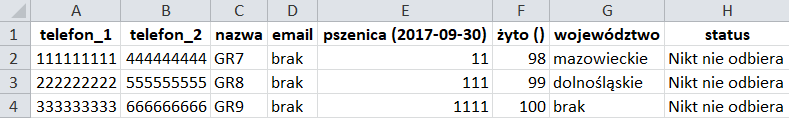
\includegraphics[width = 1\textwidth]{2.2.}
\caption{Poprawna baza do importu.}
\label{wyglad_poprawnej_bazy_do_importu}
\end{figure}
Z czego wynika konieczność dopisywania do utworzonych przez użytkownika zmiennych nawiasów z datą lub pustych nawiasów? Opiera się to na tym, że mogą się zdarzyć sytuacje, iż w badaniu przeprowadzanym w danym sezonie, nie pytano o obecny sezon, ale poprzedni lub jeszcze wcześniejszy, np. w badaniu odbywającym się w sezonie 2019/2020 zapytano respondenta o areał pszenicy w sezonie 2018/2019. W takich przypadkach przy nazwie zmiennej, w nawiasach, należy podać ostatni dzień jednego z poprzednich sezonów, do którego odnosi się dana zmienna - w bazie na rys. \ref{wyglad_poprawnej_bazy_do_importu} zmienną taką jest pszenica. Ponieważ musi to być dzień końca sezonu, dlatego jako miesiąc jest wrzesień, a jako dzień - 30. Konieczność stosowania pustych nawiasów wtedy, gdy mowa o obecnym sezonie wynika z tego, że użytkownik powinien mieć świadomość tego, co robi (pozostawienie możliwości pustego miejsca mogłoby wiązać się z tym, że zapomniano po prostu dopisać przy zmiennej nawiasu z datą), gdyż określenie dat jest ważnym elementem importu, mając kluczowe znaczenie przy wyszukiwaniu rekordów. Zatem pusty nawias oznacza, że zmienna odnosi się do obecnego sezonu i z tego też powodu program nie pozwoli, by przy jakiejś zmiennej, zamiast pustego nawiasu, była data wskazująca na ostatni dzień obecnego sezonu - mogłoby to oznaczać, że użytkownik nie do końca rozumie, jakimi zasadami powinien się kierować. W przypadku nawiasów pozostawionych jako puste, program korzysta z daty badania wpisanej w polu ,,Data badania'' - używa jej, by ocenić, czy dla obecnego sezonu, jeśli danych kontakt posiada już wartość dla tej zmiennej (np. żyta z naszego przykładu), należy ją zaktualizować czy nie. Jeśli datą badania jest 2020-05-05, natomiast w bazie rolników kontakt X posiada już wartość dla żyta z badania przeprowadzonego 2020-06-06, to zachowana zostanie wartość z badania, które odbyło się później. \par
Nieco inaczej wygląda to w przypadku informacji o województwie - jeśli do tej pory do kontaktu było przypisane określone województwo, a później zaimportowano bazę, w której znalazł się ten kontakt, lecz tym razem w miejscu województwa widniało słowo ,,brak'', to wartość ,,brak'' zostanie zignorowana. Innymi słowo, ,,brak'' w przypadku województw nigdy nie jest preferowany, bez względu na to, jak nowe byłyby te dane. \par
W trakcie importu przeprowadzany jest proces deduplikacji poprzez sprawdzanie, czy jakikolwiek numer telefonu danego kontaktu nie powtarza się z jakimkowiek numerem telefonu innego kontaktu. Jeśli tak się dzieje, to wszystkie numery telefonu są zbierane, zachowywanych jest maksymalnie dziewięć różnych numerów i wszystkie one są przypisywane do jednego kontaktu. Wszystkie wartości zmiennych zostają zachowane ze wszystkich tych kontaktów, o ile nie są sprzeczne (tj. jeśli w wyniku deduplikacji okazuje się, że kontakt w badaniu z dnia 2020-09-09 podał areał pszenicy 50 ha oraz 5 ha, to zachowana zostaje jedna, losowa wartość). Jeśli chodzi o statusy, to zachowuje się maksymalnie dwadzieścia najnowszych statusów, a dla województw - najnowsze województwo inne niż ,,brak''. W przypadku nazwy oraz emaila dla takich kontaktów, preferowane są te nazwy i emaile, które nie są słowem ,,brak''; jeśli jest takich więcej niż jeden, wybierana jest wartość losowa. Jeśli któryś z tych kontaktów był zawieszony (patrz kolejny punkt), to zawieszenie zawsze jest preferowane. \par 
Należy pamiętać, że preferowanie wartości różnych od słowa ,,brak'' ma miejsce jedynie podczas deduplikacji. Jeśli 2020-05-05 wprowadzono nowe dane dla kontaktu X, w tym zmieniono email z ,,przykladowy@email.pl'' na ,,brak'', to kontakt ten będzie miał od teraz w miejscu emaila słowo ,,brak''.
\section{Zawieszanie kontaktów}
Zawieszanie kontaktów służy jedynie do czasowego wyłączenia osób z wyszukiwania (a zatem i z udziału w badaniach). Można sobie wyobrazić sytuację, kiedy kontakt zostanie zawieszony na tak długo, że właściwie można go rozpatrywać jako zawieszonego na zawsze. Taka funkcjonalność odpowiadałaby funkcjonalności Listy Robinsona jako miejsca, gdzie odkładają się dane osób, które nie chcą kontaktu. Idea czasowego zawieszania udziału w badaniach opiera się na tym, że w wielu przypadkach nie powinno się wyłączać kogoś z badań na zawsze, ponieważ wydaje się, że często są to decyzje pochopne, podejmowane pod wpływem emocji - zarówno ankietera, jak i potencjalnego respondenta. Bardziej prawdopodobne jest bowiem, że ktoś nie życzy sobie kontaktu przez określony czas lub w określonych sytuacjach niż zawsze, bezwzględnie. \par
Zawieszanie kontaktów możliwe jest na dwa sposoby - poprzez przeszukiwanie statusów lub przeszukiwanie numerów telefonów (rys. \ref{zawieszanie_kontaktow_interfejs}). \par
\begin{figure}[h!]
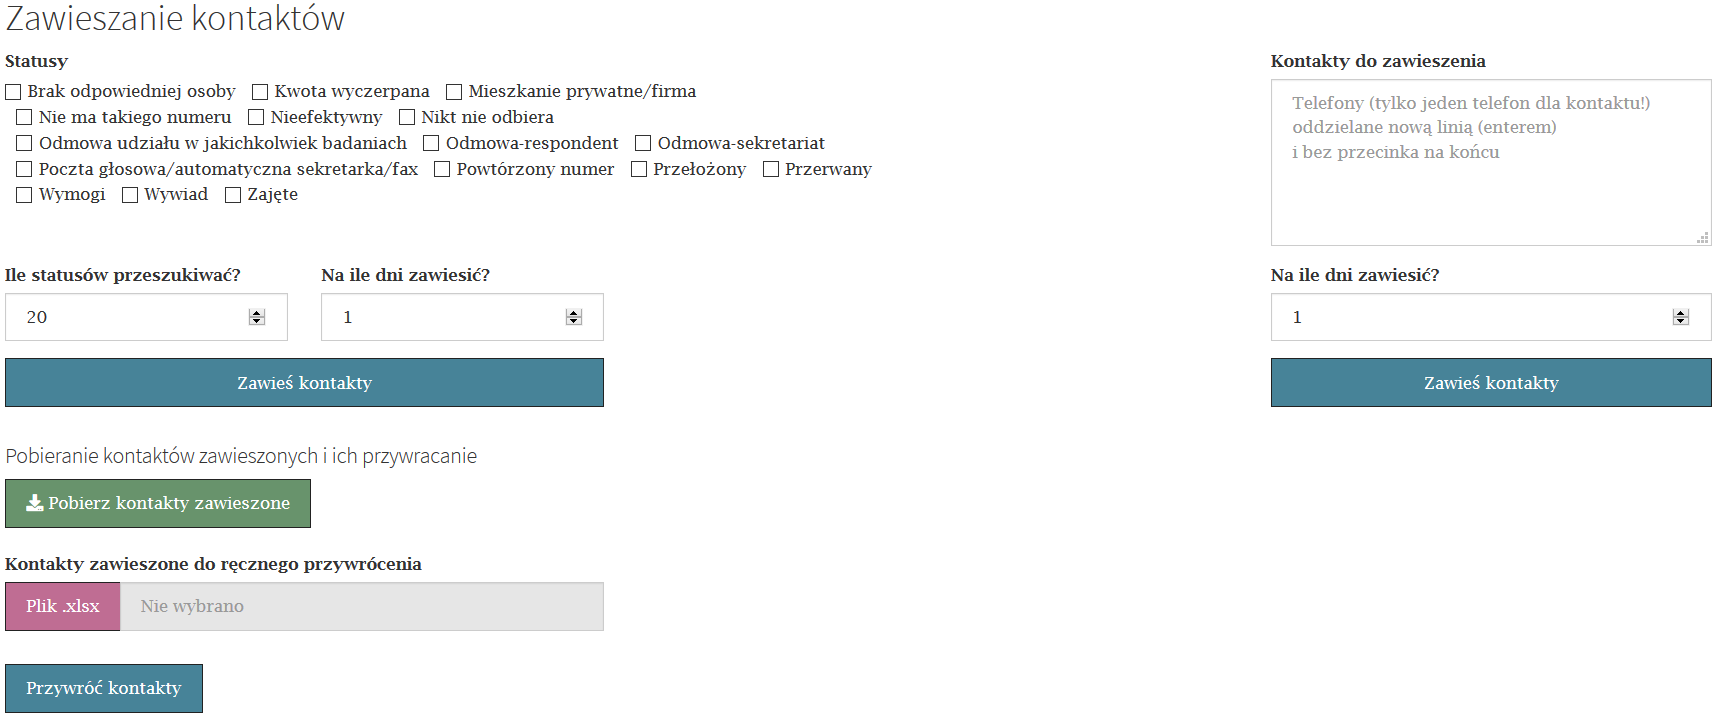
\includegraphics[width = 1\textwidth]{2.3.}
\caption{Interfejs do zawieszania kontaktów.}
\label{zawieszanie_kontaktow_interfejs}
\end{figure}
W przypadku filtrowania ważny był udział statusów, natomiast w przypadku zawieszania określa się, które statusy jako jedyne mogą wystąpić w tylu maksymalnie najnowszych statusach dla danego kontaktu, ile określono w polu ,,Ile statusów przeszukiwać?''. Jeśliby np. zaznaczono statusy ,,Odmowa udziału w jakichkolwiek badaniach'' oraz ,,Odmowa-respondent'' i pozostawiono resztę pól z wartościami domyślnymi, tj. przeszukiwanie dwudziestu statusów i zawieszenie na jeden dzień, to na jeden dzień zawieszone zostaną te kontakty, w których we wszystkich statusach (ponieważ kontakt może mieć przypisanych maksymalnie dwadzieścia statusów) były tylko wartości ,,Odmowa udziału w jakichkolwiek badaniach'' lub ,,Odmowa-respondent''. Jeśli w choć jednym z tych dwudziestu statusów zdarzyłaby się inna wartość, kontakt nie zostanie zawieszony. \par
Gdy chcemy zawiesić konkretną osobę, musimy znać choć jeden numer telefonu do niej przynależny. Nie ma powodu wypisywać więcej niż jednego numeru, ale gdyby tak się stało, to program zadziała poprawnie. \par
Dla kontaktów zawieszonych wciąż można importować nowe dane. Może się np. zdarzyć, że osoba, która jest zawieszona, jakimś sposobem znajdzie się w bazie do badania i weźmie w nim udział. Taki rekord wciąż można zaimportować i zostanie on zaktualizowany o nowe dane. To nie zmieni jednak jego stanu zawieszenia. \par
Mimo że monitorowanie upływu czasu zawieszenia dokonywane jest automatycznie, to wciąż można ręcznie przywrócić zawieszone kontakty. By to zrobić, najpierw najlepiej pobrać kontakty zawieszone (przycisk ,,Pobierz kontakty zawieszone''), ponieważ pozwoli to nie tylko mieć podgląd na wszystkie kontakty o takiej charakterystyce, ale również stworzy plik o strukturze, która jest konieczna do przywrócenia zawieszonych kontaktów (rys. \ref{zawieszanie_kontaktow_pobrany_plik}). \par
\begin{figure}[h!]
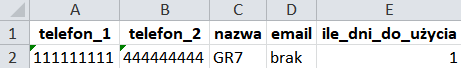
\includegraphics[width = 0.5\textwidth]{2.4.}
\centering
\caption{Plik z informacją o zawieszonych kontaktach.}
\label{zawieszanie_kontaktow_pobrany_plik}
\end{figure}
W pobranym arkuszu znajdą się wszystkie kolumny z telefonami, nazwa, email oraz informacja, ile pozostało dni do tego, by kontakt mógł być ponownie wyszukiwany. By usunąć kogoś z listy kontaktów zawieszonych, wystarczy pozostawić w tym pliku interesujące nas rekordy i wczytać go, naciskając następnie przycisk ,,Przywróć kontakty''. Minimalna struktura pliku wymagana przy tej operacji to arkusz z kolumną ,,telefon\textunderscore 1'' oraz jakiekolwiek dane w tej kolumnie. Nie trzeba zatem zachowywać dokładnie takiej struktury, jak w pobranym pliku, choć posłużenie się uprzednio pobranymi danymi wydaje się najłatwiejsze.
\section{Usuwanie kontaktów i telefonów}
Usuwanie odpowiada sytuacji, kiedy sam użytkownik nie chce w bazie danych określonych osób lub numerów telefonów lub też osoba, której dane znajdują się w bazie, chce ich usunięcia - w całości lub poszczególnych numerów telefonów. Usunięcie takie nie gwarantuje, że numer telefonu, a zatem też kontakt, nie pojawi się ponownie (np. w wyniku importu jakiegoś starego badania lub ponownego odnalezienia tych danych w innych bazach, np. w Internecie). \par
\begin{figure}[h!]
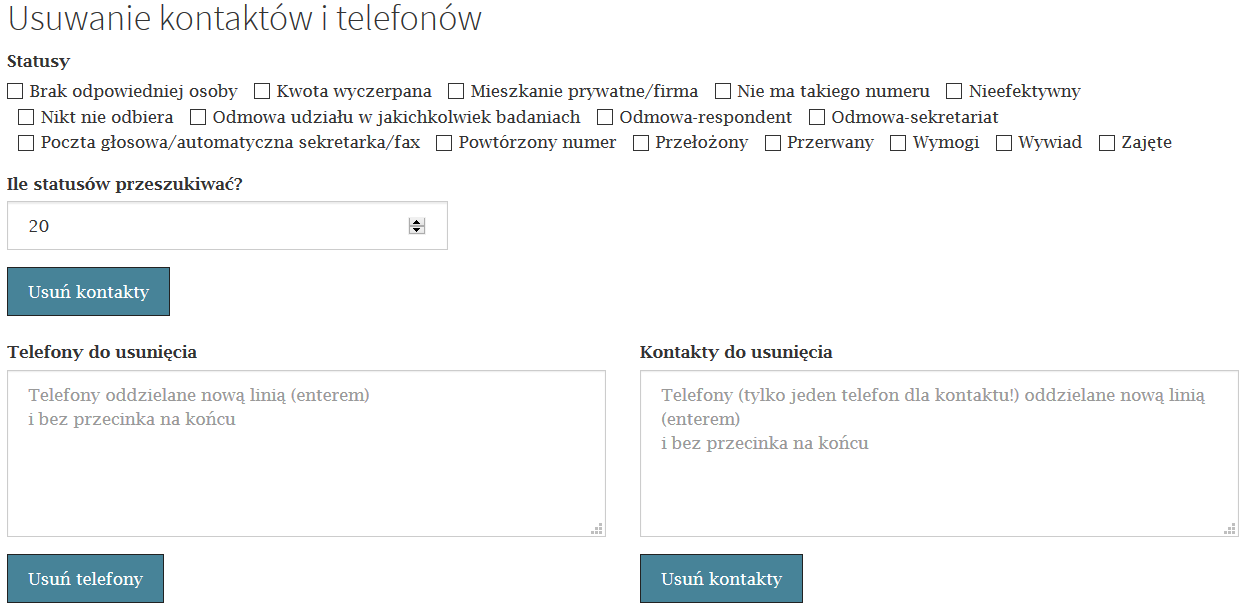
\includegraphics[width = 1\textwidth]{2.5.}
\centering
\caption{Interfejs do usuwania kontaktów i telefonów.}
\label{usuwanie_kontaktow_telefonow_interfejs}
\end{figure}
Przeszukiwanie poprzez przeglądanie statusów opiera się na tej samej zasadzie, jak w przypadku zawieszania kontaktów - wszystkie wybrane statusy i tylko one muszą wystąpić w najnowszych tylu maksymalnie statusach, jaką liczbę wpisano w polu ,,Ile statusów przeszukiwać?'' (rys. \ref{usuwanie_kontaktow_telefonow_interfejs}). \par
W przypadku usuwania numerów telefonów ważne jest pamiętanie o jednej rzeczy - jeśli usunięto numer telefonu, który jako jedyny widniał przy danym kontakcie, to cały ten kontakt zostanie usunięty z bazy danych. \par
Podobnie, jak w przypadku zawieszania kontaktów, w razie chęci usunięcia kontaktu na podstawie numeru telefonu, nie ma potrzeby wypisywania więcej niż jednego numeru telefonu dla tego kontaktu, choć takie działanie również przyniesie pożądany efekt.
\chapter{Modyfikacja zmiennych}
\thispagestyle{empty}
\pagebreak
\section{Dodawanie/zmienianie opisu zmiennych}
Choć zmienne powinny mieć możliwie najbardziej informacyjne nazwy, to jednocześnie nie powinny być zbyt długie. Etykiety (opisy) pomagają wytłumaczyć użytkownikowi, co dokładnie oznacza dana zmienna. Zmienna ,,ma\textunderscore email'', mimo że tworzona automatycznie, nie posiada etykiety. Użytkownik może taką stworzyć na podstawie informacji zamieszczonych w sekcji ,,Wyszukiwanie zmiennych'', choć nazwa zmiennej w połączeniu z wartościami, jakie przyjmuje, wydaje się wystarczająco jasna. \par
\begin{figure}[h!]
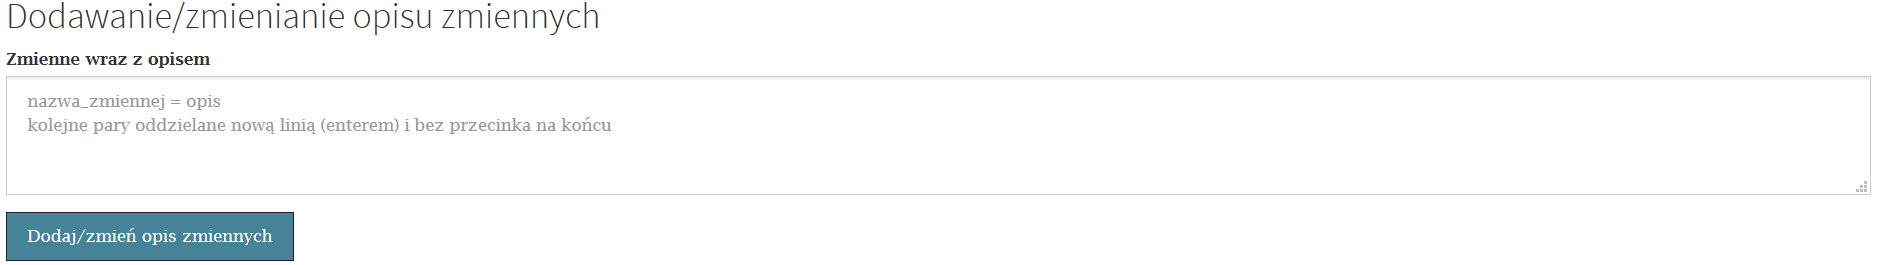
\includegraphics[width = 1\textwidth]{3.1.}
\caption{Interfejs do dodawania/zmieniania opisu zmiennych.}
\label{dodawanie_usuwanie_opisu_zmiennych_interfejs}
\end{figure}
Etykiety można tworzyć, zmieniać oraz usuwać. Usuwanie  odbywa się poprzez przypisanie zmiennej pustej etykiety, np. \par
\begin{center}
pszenica = 
\end{center}
Zmiennych oraz opisów nie zamyka się w cudzysłów.
\section{Zmienianie nazw zmiennych}
Zmiana nazwy zmiennej może być podyktowana dwoma powodami - najbardziej oczywista jest sytuacja, kiedy jest to po prostu chęć posiadania zmiennej o innej nazwie. Zmiana nazwy może prowadzić jednak również do agregowania zmiennych. \par
\begin{figure}[h!]
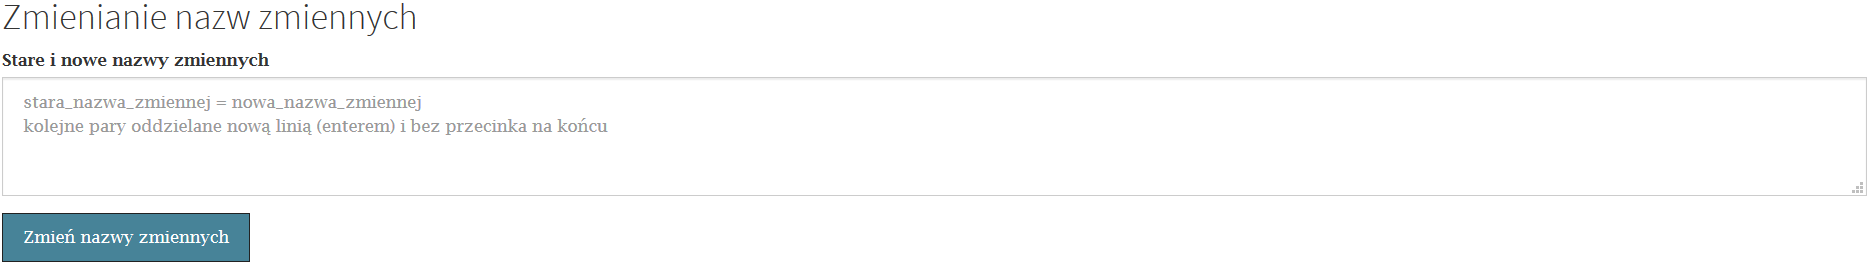
\includegraphics[width = 1\textwidth]{3.2.}
\caption{Interfejs do zmieniania nazw zmiennych.}
\label{zmienianie_nazw_zmiennych_interfejs}
\end{figure}
Jako przykład niech posłuży zmienna ,,pszenica'' oraz ,,żyto''. Załóżmy, że w badaniu z 2020-05-05 kontakt X miał 5 ha pszenicy, a w badaniu z 2020-06-06 ten sam kontakt miał 50 ha żyta. Zmiana nazwy zmiennej ,,pszenica'' na ,,żyto'' sprawi, że od teraz kontakt X będzie miał 5 ha żyta z badania wykonanego 2020-05-05 oraz 50 ha żyta z badania z dnia 2020-06-06. Ponieważ oba te badania odbyły się w tym samym sezonie, to zachowana zostanie wyłącznie nowsza informacja, zatem po zmianie nazwy zmiennej, utracone zostaną dane o tym, że kontakt X w badaniu z 2020-05-05 miał 5 ha żyta (oryginalnie: pszenicy). Do podobnej utraty informacji dojdzie, jeśli np. kontakt Y w badaniu z 2020-04-04 miał 1 ha pszenicy oraz w tym samym badaniu miał 10 ha żyta. Wtedy, po zmianie nazwy zmiennej ,,pszenica'' na ,,żyto'', tylko jedna z tych zmiennych zostanie zachowana (ponieważ nie można mieć dwóch różnych wartości tej samej zmiennej z danego dnia czy sezonu) - program losowo odrzuci jedną wartość. \par
Istnieje ograniczenie na to, jakie nazwy zmiennych można zmieniać - próba zmiany nazwy zmiennych ,,status'' lub ,,województwo'' bądź próba zmiany nazwy jakiejś innej zmiennej na którąś z tych dwóch nazw zakończy się błędem. Ponadto, nie można zmienić nazwy zmiennej ,,ma\textunderscore email'', choć możliwa jest zmiana nazwy innej zmiennej na ,,ma\textunderscore email''. Nie można także używać niedozwolonych znaków w nazwie zmiennej - zastosowanie mają tu te same ograniczenia, jak przy imporcie bazy (tylko cyfry, litery, podkreślenie). \par
Nie zapisuje się nazw zmiennych z użyciem cudzysłowu.
\section{Rekodowanie odpowiedzi}
Pomimo możliwości agregowania za pomocą zmieniania nazw zmiennych, jest już raczej jasne, że nie jest to bezpieczny sposób modyfikacji i użytkownik powinien korzystać z takich rozwiązań z dużą świadomością tego, jakie będą konsekwencje. Bezpieczniejszym rozwiązaniem jest posłużenie się funkcjonalnością ,,Rekodowanie odpowiedzi'', choć trzeba pamiętać, że w pewnych przypadkach określone operacje i tak będą możliwe jedynie poprzez zmienianie nazw zmiennych. \par
\begin{figure}[h!]
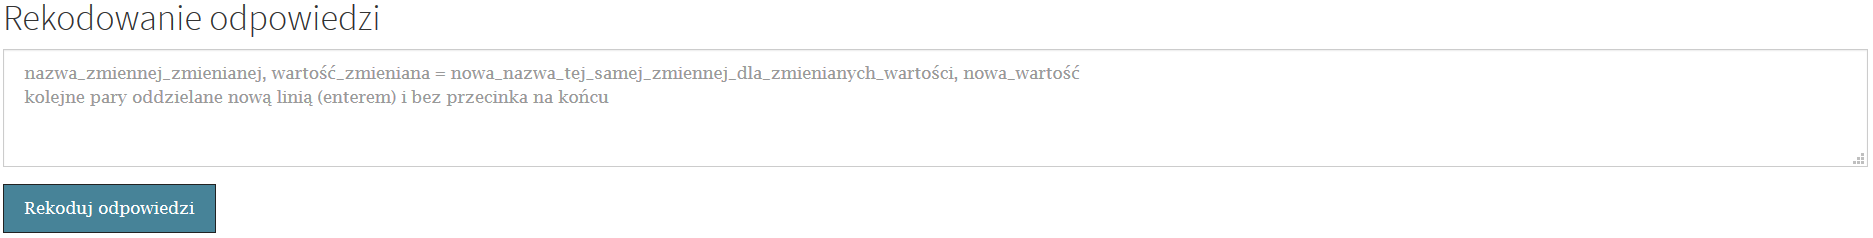
\includegraphics[width = 1\textwidth]{3.3.}
\caption{Interfejs do rekodowania odpowiedzi.}
\label{rekodowanie_odpowiedzi_interfejs}
\end{figure}
Rekodowanie odpowiedzi służy wyłącznie do zmiany nazwy zmiennej i określonych wartości tej zmiennej na inną nazwę zmiennej dla tych wartości lub po prostu na inaczej nazwane wartości, bez zmieniania nazwy zmiennej. Nadaje się do rekodowania zmiennych ilościowych i jakościowych, choć funkcjonalność ta powstała wyłącznie z myślą o zmiennych jakościowych. Wynika z tego następujące ograniczenie:
\begin{itemize}
\item w przypadku rekodowania odpowiedzi dla zmiennych ilościowych, istnieje wyłącznie możliwość zmiany konkretnych, poszczególnych wartości, np. 1 ha pszenicy na 10 ha pszenicy. Nie ma zatem możliwości tworzenia np. nowej zmiennej, która będzie zawierać przedziały dla jakiejś zmiennej ilościowej. Jest to podyktowane tym, że baza rolników została pomyślana raczej jako narzędzie do przechowywania danych w możliwie surowej formie, tj. aby użytkownik nie tworzył ogólnych zmiennych tam, gdzie da się stworzyć zmienne szczegółowe. Zmienna przechowująca informacje o areale pszenicy w przedziałach jest na bardziej ogólnym poziomie pomiaru niż zmienna przechowująca konkretne wartości areału pszenicy. Oczywiście, jeśli przeprowadzono badanie, w którym tylko w ten sposób pytano o pszenicę, to taką zmienną można zaimportować do programu, ale jeśli w programie istnieje zmienna szczegółowa, to nie powinno się tworzyć dodatkowej, bardziej ogólnej zmiennej. Mogłoby to ułatwiać późniejsze filtrowanie, ale nie sprawiałoby, że jakieś filtrowanie, które wcześniej nie było możliwe, teraz takie jest. To ograniczenie zostało stworzone po to, by aplikacja była bardziej wydajna, ponieważ im więcej rekordów w bazie, a zatem im więcej zmiennych, tym na większym wolumenie danych trzeba operować.
\end{itemize}
Najważniejsze w zrozumieniu, jak odbywa się rekodowanie odpowiedzi, jest zdanie sobie sprawy z tego, co dzieje się z nazwą zmiennej wtedy, gdy, podczas rekodowania odpowiedzi, zmieniamy jej nazwę. Na rys. \ref{rekodowanie_fragment_bazy_rolnikow} przedstawiono fragment bazy rolników - takiej, jaka jest przechowywana w aplikacji. \par
\begin{figure}[h!]
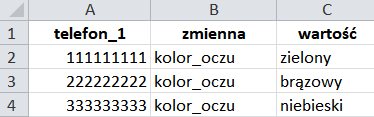
\includegraphics[width = 0.5\textwidth]{3.7.}
\centering
\caption{Uproszczony fragment bazy rolników.}
\label{rekodowanie_fragment_bazy_rolnikow}
\end{figure}
Składnia poprawnego wyrażenia rekodującego odpowiedzi wygląda w ten sposób: ,,Stara nazwa zmiennej, wartość zmieniana = Nowa nazwa zmiennej dla zmienianych wartości, nowa wartość''. Wyrażenie ,,Nowa nazwa zmiennej dla zmienianych wartości'' oznacza, że nie dochodzi do zmiany nazwy zmiennej, ale jedynie zmiennej dla określonych wartości. Gdy jako przykład wziąć zmienną kolor\textunderscore oczu i chcieć zmienić wartość ,,zielony'' na ,,turkusowy'', jednocześnie zmieniając nazwę zmiennej na ,,kolor\textunderscore stawu\textunderscore respondenta'', należy zapisać to w ten sposób: \par
\begin{center}
kolor\textunderscore oczu, zielony = kolor\textunderscore stawu\textunderscore respondenta, turkusowy
\end{center}
Wartości zmiennych nie są zapisywane z użyciem cudzysłowu, inaczej niż przy filtrowaniu. Użycie cudzysłowu sprawiłoby, że program nie odnalazłby żadnej wartości i nie doszłoby do zmiany. Powyższe polecenie przekształci bazę na postać widoczną na rys. \ref{po_rekodowaniu_fragment_bazy_rolnikow}.
\begin{figure}[h!]
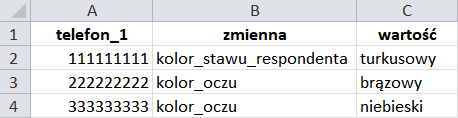
\includegraphics[width = 0.5\textwidth]{3.8.}
\centering
\caption{Uproszczony fragment bazy rolników po rekodowaniu odpowiedzi.}
\label{po_rekodowaniu_fragment_bazy_rolnikow}
\end{figure}
Widać, że nazwa zmiennej zmienia się wyłącznie dla tych wartości (odpowiedzi), które rekodujemy. Jeśli chcemy zachować poprzednią nazwę zmiennej, trzeba po prostu wpisać jej obecną nazwę, a nie nową. \par
Rekodowanie odpowiedzi również pozwala agregować zmienne i również wiąże się to z tymi samymi konsekwencjami w możliwej utracie informacji, jak w przypadku zmiany nazwy zmiennej. Podobnie, ograniczono możliwość używanych nazw zmiennych - nie można w nazwach zmiennych używać słów ,,status'' czy ,,województwo'' oraz nie można w nowej nazwie zmiennej użyć niedozwolonych znaków - możliwe są tylko litery, cyfry, podkreślenie. Nie da się także zmienić nazwy zmiennej ,ma\textunderscore email''. \par
W nazwach zmiennych, ale również w nazwach wartości - a więc inaczej niż w przypadku filtrowania - nie używa się cudzysłowu.
\section{Dodawanie i usuwanie zmiennych bez historii}
Dla każdej zmiennej jej dane historyczne nie mogą być bardziej szczegółowe niż wyznaczane przez koniec i początek sezonu - jeśli zmienna posiada historię, jest to historia, w której obserwacja wydarza się raz w sezonie. Logika sezonowości nie jest jednak odpowiednia dla wszystkich zmiennych - można sobie wyobrazić, że zmienna ,,województwo'', opisująca miejsce, w którym znajduje się gospodarstwo rolne, nie tylko nie zmienia się co sezon, ale może nawet w ogóle się nie zmienia dla danego kontaktu. \par
 \begin{figure}[h!]
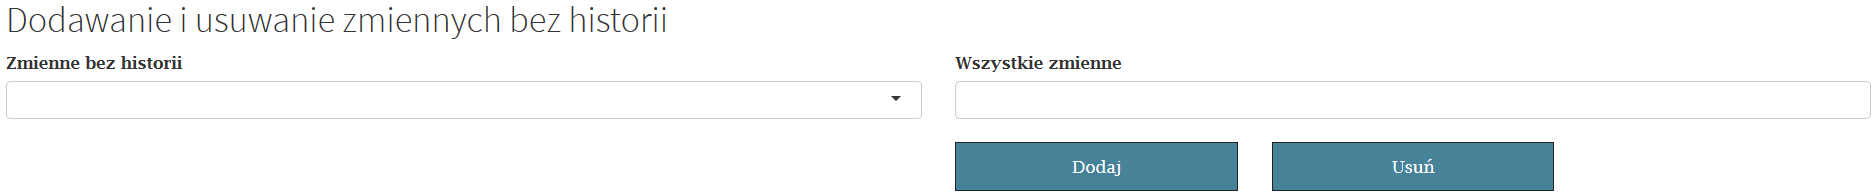
\includegraphics[width = 1\textwidth]{3.4.}
\caption{Interfejs do dodawania i usuwania zmiennych bez historii.}
\label{dodawanie_usuwanie_zmiennych_bez_historii_interfejs}
\end{figure}
Choć można by sobie wyobrazić wiele różnych stanów, które dla różnych zmiennych byłyby odpowiednie, to w programie dopuszczono tylko dwie możliwości: zmienna nie posiada historii lub posiada historię wyznaczaną przez sezony. Nie chodzi jednak o to, by zastanawiać się, jaki fragment świata powinien mieć historię, a jaki nie - z pewnością wiele, o ile nie wszystkie zmienne, mogłyby posiadać historię. Z drugiej strony, im mniej danych historycznych w bazie, tym bardziej wydajna powinna ona być. Ustalając, czy dana zmienna powinna mieć historię, należy odpowiedzieć na pytanie: czy dane historyczne dla tej zmiennej będą potrzebne? \par
Dane historyczne przydają się wtedy, gdy wiemy, że kontakt kiedyś spełniał kryterium wyszukiwania, później nie spełniał, a obecnie nie mamy informacji, czy je spełnia. Przy jakich zmiennych możemy założyć, że jest istotna szansa, iż obecnie kontakt spełni kryterium wyszukiwania (kryterium zakwalifikowania do badania, do którego szukamy respondentów)? Jeśli jako przykład wybrać zmienną ,,ma\textunderscore email'', to jaka jest szansa, że ktoś, mający kiedyś adres email, później niemający, obecnie będzie go miał, tj. jaka jest szansa, że (1) ktoś mógłby mieć adres email, a później nie mieć go wcale; (2) ktoś, kto miał adres email, później nie miał go wcale, będzie go miał znów? Jeśli w obu tych przypadkach uznajemy szansę za tak małą, że nieznaczącą dla nas, warto dodać zmienną do zbioru zmiennych bez historii. \par
Zmienne w tym zbiorze są aktualizowane najnowszą wartością przy imporcie, a wartość poprzednia nie odkłada się w bazie danych. Decyzję o dopisaniu zmiennej do zmiennych bez historii można cofnąć w dowolnym momencie - tak, jak w dowolnym momencie można zmienną dopisać - ale historia, która została skasowana (w wyniku wcześniejszego dodania zmiennej do zmiennych bez historii), nie będzie przywrócona. \par
Na rys. \ref{dodawanie_usuwanie_zmiennych_bez_historii_interfejs} przedstawiono interfejs opisywanej funkcjonalności. Po lewej widoczna jest lista zmiennych bez historii, natomiast po prawej stronie lista wygląda nieco inaczej - mimo że wydaje się pusta, po kliknięciu na nią pokażą się wszystkie zmienne w bazie rolników. Za jednym razem można wybrać więcej niż jedną zmienną, zatem za jednym razem można dodawać lub usuwać z listy zmiennych bez historii więcej niż jedną zmienną.
\section{Usuwanie danych na podstawie zmiennej i daty}
Wiele razy wspominano do tej pory o wydajności aplikacji, w tym o tym, że zależy ona od wielkości bazy danych. Wielkość z kolei zależy w największym stopniu od liczby zmiennych i tego, jak bardzo historyczne dane są przechowywane. Zakłada się bowiem, że przyrost liczby zmiennych (i ich historii) będzie szybszy niż przyrost nowych kontaktów do bazy. \par
 \begin{figure}[h!]
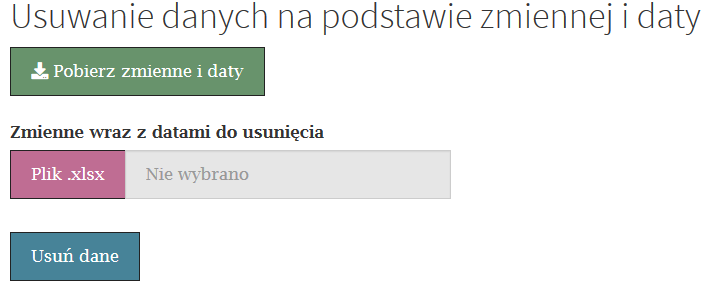
\includegraphics[width = 0.8\textwidth]{3.5.}
\centering
\caption{Interfejs do usuwania danych na podstawie zmiennej i daty.}
\label{usuwanie_danych_na_podstawie_zmiennej_daty_interfejs}
\end{figure}
Wtedy, gdy od pewnego momentu czasu (a dokładniej: sezonu) dane dla określonej zmiennej przestają mieć wartość, ze względów wydajnościowych powinno się usuwać takie rekordy. Usuwanie nie jest możliwe dla zmiennej ,,województwo'' - zmienna ta i tak nie przechowuje historii - oraz dla zmiennej ,,status'' (bez względu na to, jak stare są informacje o statusie, maksymalnie 20 statusów będzie zachowywanych). Usuwanie odbywa się poprzez wczytanie pliku zawierającego tylko dwie kolumny: ,,zmienna'' i ,,sezon'', w takiej właśnie kolejności. Plik taki jest tworzony podczas pobierania zmiennych i dat (przycisk ,,Pobierz zmienne i daty'', rys. \ref{usuwanie_danych_na_podstawie_zmiennej_daty_interfejs}). Wygląd pobranego pliku przedstawia rys. \ref{pobrany_plik_usuwanie_danych_na_podstawie_zmiennej_daty}. \par
 \begin{figure}[h!]
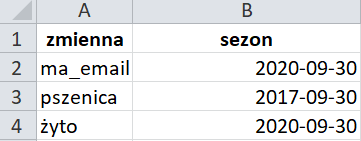
\includegraphics[width = 0.5\textwidth]{3.6.}
\centering
\caption{Pobrany plik ze zmiennymi i datami (sezonami).}
\label{pobrany_plik_usuwanie_danych_na_podstawie_zmiennej_daty}
\end{figure}
W celu usunięcia zmiennych dla danych sezonów, trzeba pozostawić je w pliku, tj. pobrany wcześniej plik należy wczytać ponownie, pozostawiając w nim te zmienne i te sezony dla danej zmiennej, które chcemy usunąć z bazy danych i nacisnąć przycisk ,,Usuń dane''. \par
W poprzednim punkcie dyskutowana była kwestia zmiennych bez historii. Teraz warto zauważyć, że zmienne bez historii zawsze jako sezon będą mały podany obecny sezon, choć to naturalnie nie znaczy, że jeśli przy zmiennej widnieje wyłącznie obecny sezon, to jest to zmienna bez historii.
\chapter{Kopia oraz wydajność bazy}
\thispagestyle{empty}
\pagebreak
\section{Zapisywanie i przywracanie kopii}
Aplikacja rozróżnia dwa rodzaje kopii - kopię stworzoną przez użytkownika oraz kopie stworzone automatycznie. Ta pierwsza jest tylko jedna - każda kolejna kopia użytkownika nadpisuje poprzednią. Kopie automatyczne tworzone są natomiast co dwa tygodnie i przechowywane przez pół roku. Z poziomu aplikacji możliwe jest zapisanie kopii użytkownika, przywrócenie kopii użytkownika oraz przywrócenie dowolnej istniejącej kopii automatycznej. \par
 \begin{figure}[h!]
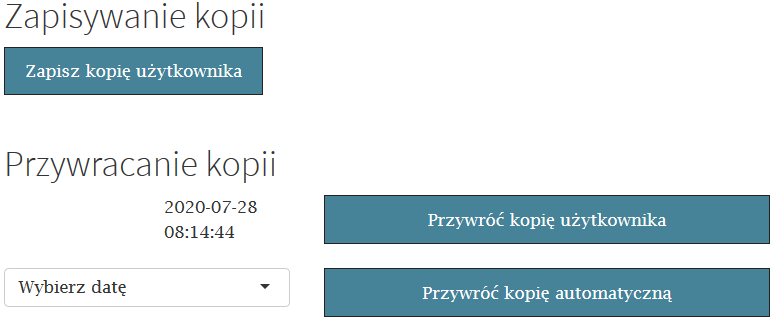
\includegraphics[width = 0.8\textwidth]{4.1.}
\centering
\caption{Interfejs do zapisywania i przywracania kopii.}
\label{zapisywanie_przywracanie_kopii_interfejs}
\end{figure}
Kopie nie służą do ochrony przed awariami technicznymi, jak np. zniszczenie dysku twardego, na którym przechowywana jest baza danych, ponieważ znajdują się na tym samym dysku. Ich celem jest jedynie możliwość powrotu do stanu poprzedniego wtedy, gdy użytkownik podjął akcję, której konsekwencje okazały się negatywne. Zapisanie kopii użytkownika pozwala stworzyć kopię tuż przed podjęciem takiej akcji, natomiast kopie automatyczne pozwalają wrócić do poprzedniego stanu w sytuacjach, gdy błąd zauważono później. \par
Myśląc o bezpieczeństwie danych oraz o stanie bazy wolnym od błędów, trzeba zdać sobie sprawę z tego, że aplikacja ,,Baza rolników'' jest niczym więcej, jak programem, który dokonuje transformacji danych. To dane wprowadzane do programu są cenne, a nie dane, które uległy obróbce. Oznacza to, że kluczowe jest nie tyle zabezpieczenie bazy przechowywanej przez program, ile zabezpieczenie danych, które użytkownik przygotował w celu zaimportowania do aplikacji. To one powinny być przetrzymywane w bezpiecznym miejscu, ponieważ gdyby nawet baza przechowywana przez program uległa zniszczeniu, wystarczy ponownie zaimportować dane, co przy nawet dużej ich liczbie nie powinno zająć więcej niż kilku godzin. Oczywiście, sam kod aplikacji również powinien być przechowywany w takim miejscu, choć dane gotowe do importu są ważniejsze - można by z nich bowiem korzystać nawet wtedy, gdy ta aplikacja nie istniałaby. \par
Kopia użytkownika jest zapisana wtedy, gdy wyświetlają się - widoczne na rys. \ref{zapisywanie_przywracanie_kopii_interfejs} - data i czas ostatniego zapisu (obok przycisku ,,Przwróć kopię użytkownika''). Puste miejsce oznaczałoby, że do tej pory nie stworzono takiej kopii. \par
Ważne jest, gdy mowa o kopiach, jeszcze jedna sprawa - dostęp wielu użytkowników w tym samym czasie do aplikacji. Jedną z możliwości działania aplikacji jest uruchomienie jej na serwerze, dzięki czemu wielu użytkowników w tym samym czasie może z niej korzystać. ,,W tym samym czasie'' oznacza, że użytkownicy nie blokują sobie wejść do aplikacji, ale nie oznacza, że możliwe jest dokonywanie operacji równolegle. Jeśli użytkownik X importuje nowe dane do bazy i zajmuje to 20 sekund, to przez ten czas użytkownik Y nie otrzyma wyników wyszukiwania i dopiero po tym, gdy operacja zlecona przez użytkownika X zakończy się, program zacznie przetwarzać polecenie użytkownika Y. Wszyscy użytkownicy dzielą jedno środowisko - w przykładzie powyżej, użytkownik Y będzie dokonywał filtrowania na bazie danych przekształconej chwilę wcześniej przez użytkownika X. Dzielą jednak także kopie bazy. Może się więc zdarzyć, że użytkownik X stworzył kopię, dokonał modyfikacji i od razu po tym użytkownik Y stworzył kopię. W takiej sytuacji nie istnieje już kopia użytkownika stworzona przed modyfikacją, której dokonał użytkownik X, ale po jego modyfikacji. Sprawia to, że, mimo możliwości korzystania wielu użytkowników z aplikacji, wprowadzanie zmian do bazy nie powinno odbywać się przez więcej niż jedną osobę w tym samym czasie lub w krótkich odstępach czasu. Zagrożenia takie nie istnieją, gdy użytkownicy jedynie wyszukują dane.
\section{Dodatkowe uwagi o wydajności bazy}
Oprócz tego, co do tej pory zostało powiedziane o szybkości działania aplikacji, warto wymienić jeszcze jedną rzecz. Po każdej modyfikacji bazy, jest ona nie tylko aktualizowana w pamięci tymczasowej i udostępniania wszystkim użytkownikom korzystającym w tym czasie z programu, ale zapisywana na dysk. Szybkość zapisu zależy od kilku czynników. Bezpośrednio od wielkości bazy, ale także od szybkości dysku, liczby wątków procesora oraz wykorzystywanych w tym celu algorytmów. Aplikacja ,,Baza rolników'' ma dwie wersje - jedną przeznaczoną na system Linux (jest to jednocześnie wersja, która nadaje się do działania na serwerze, choć go nie wymaga) oraz na system Windows. Obie wykorzystują odmienne funkcje do zapisu i odczytu. Z powodów związanych z kodowaniem znaków, wersja na system Linux jest o wiele szybsza. W przypadku dobrych dysków SSD, wielu dostępnych wątkach procesora i systemu Linux czas zapisu dużej bazy powinien wynosić kilka sekund, natomiast czas ten ulegnie wydłużeniu przy wolniejszych dyskach, mniejszej liczbie wątków procesora i systemu Windows do kilkudziesięciu sekund lub więcej. Sprawia to, że, modyfikując bazę, lepiej wykonywać operacje w jednym kroku, tzn. jeśli chcemy np. usunąć kilka numerów telefonów, zawiesić kilka osób lub dodać kilka opisów zmiennych, kolejne telefony lub pary zmienna-opis lepiej wpisać w odpowiednie pole za jednym razem, oddzielić nową linią i wykonać pożądane działanie. Jeśli robilibyśmy to w osobnych krokach, baza po każdym z nich byłaby zapisywana. \par
Czas wczytania bazy jest dłuższy niż czas zapisu, ale baza nie jest ponownie wczytywana po każdej modyfikacji. Dzieje się tak tylko wtedy, gdy aplikacja na serwerze została wyłączona (celowo lub np. z racji zaniku prądu) lub zamrożona z tego powodu, że przez określony czas nikt z niej nie korzystał oraz wtedy, gdy przywracana jest któraś z kopii. Możliwe jest jednak ustawienie, aby aplikacja nigdy nie wchodziła w stan zamrożenia. Wczytywanie aplikacji (czyli wchodzenie na link) nie będzie się wtedy wiązać z nadmiernymi opóźnieniami wynikającymi z ładowania bazy do programu.
\end{document}